%\documentclass{article}
%\usepackage{graphicx,subfigure}
%\begin{document}

\begin{figure}[!h]
  \centering
   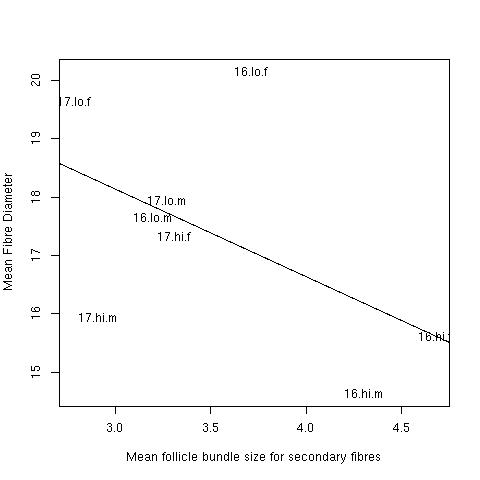
\includegraphics[width=1.0\textwidth]{1617bundledia.png}
  \caption{Plot of mean follicle bundle size for secondary fibres against mean fibre diameter for six sheep of each sex representing the four selection lines Fr+, Fr-, Fp+, Fp-. The solid line is a regression of diameter on bundle size ( Diam = 22.62 - 1.497 * Size). The multiple correlation squared is 0.27. The regression is not significant.}
  \label{fig:1617bundledia}
\end{figure}

%\end{document}

